% Provenance (never printed): see sources/outline_sources.md (Year 3:
% critical-taper theory; fold-and-thrust belts; exhumation and
% thermochronology). Brief: sources/book5/BRIEFS.md, ch. 10. Curves from
% figdata/bachelor-3/fault_bend.py, critical_taper.py and age_elevation.py.
% Exercise and problem values in the Book 5 scratch calculator calc/ch10.py.
\chapter{أحزمة الصدوع الزاحفة وأسافين التكوّن الجبلي}\label{ch:b3:orogenic-wedges}

إذا دُفعت جرّافة إلى رمل رطب أو ثلج، تراكم وتدٌ من المادة
أمام الشفرة. تتشوّه حتى يبلغ سطحها ميلًا معيّنًا؛
ومن عندها تنزلق إلى الأمام كتلةً واحدةً وتنمو بالشكل نفسه،
وتضمّ مادةً جديدةً عند طرفها الأمامي. وتسلك الأجزاء الخارجية لأحزمة الجبال،
من تايوان إلى سفوح الألب، السلوك نفسه: فهي أسافين من صخور كُشطت عن صفيحة
ودُفعت فوق قاعدة ضعيفة، ويدلّ كلٌّ من ميل سطحها وانحدار قاعدتها
على مدى ضعف تلك القاعدة، وعلى ارتفاع
ضغط الموائع داخلها. يبني هذا الفصل هندسة أحزمة الصدوع الزاحفة،
وميكانيكا الوتد، والساعات التي تقيس سرعة صعود صخوره
إلى السطح.
% ledger: dsd83:taper

\begin{recall}
ترد الصدوع الزاحفة والانحياز وهندسة الطيّات في مجلد السنة الأولى، في
فصله عن الصدوع والطيّات والنسيج؛ ومعيار كولومب، وقانون بيرلي، والإجهاد
الفعّال ونسبة ضغط المسامات $\lambda = P/\sigma_v$ في فصله عن
الإجهاد والانفعال والريولوجيا؛ ودرجة حرارة الإغلاق وعمر التبريد
ترد في فصله عن طرائق التأريخ الإشعاعي. وسطح الانفصال وحزام الطيّات
والصدوع الزاحفة، والتكتونيات ذات القشرة الرقيقة والسميكة، والمقطع العرضي
المتوازن ترد في مجلد السنة الثانية، في فصله عن تشريح
السلسلة الجبلية؛ والاستخراج ومعدّله في فصله عن مسارات P--T--t. وبناء
الانحناء الزاوي والمساحة الفائضة $A = Sh$ لطيّةٍ فوق
الانفصال ترد في \cref{ch:b3:structural-analysis}؛ \omterm{def:b3:lithosphere-thermal-models:peclet}{وعدد بيكليه الحراري} في
\cref{ch:b3:lithosphere-thermal-models}.
\end{recall}

\section{هندسة الصدوع الزاحفة}\label{sec:b3:orogenic-wedges:geometry}

لا يقطع الصدع الزاحف المتتابعة الطبقية على مستوٍ واحد مستقيم.
فهو يتبع طبقةً ضعيفةً، كالطَّفل أو صخرًا تبخّريًا، مسافاتٍ طويلة، ثم
يتسلّق بحدّة عبر الطبقات القوية فوقها حتى الطبقة الضعيفة التالية.
ويتحكّم هذا السُّلّم الذي يرسمه في طيّات الجدار المعلّق.

\begin{definition}[المنحدر، والسطح المستوي، والدوبلكس، والصدع الزاحف خارج التسلسل]\label{def:b3:orogenic-wedges:thrust-geometry}
\emph{السطح المستوي للصدع الزاحف}\index{السطح المستوي للصدع الزاحف} هو قطعةٌ من الصدع الزاحف تمتدّ
موازيةً للطبقية، عادةً في طبقةٍ ضعيفة؛ و\emph{المنحدر
للصدع الزاحف}\index{المنحدر للصدع الزاحف} قطعةٌ تقطع الطبقية،
عادةً بزاوية بين 20 و\ang{30}، تصل سطحًا مستويًا سفليًّا بآخر علويّ.
و\emph{الدوبلكس للصدع الزاحف}\index{الدوبلكس للصدع الزاحف} تكدّسٌ من شرائح محدودة بصدوع،
تُسمّى الأحصنة، محصورةً بين صدع زاحف قاعدي من الأسفل وصدع زاحف سقفي
من الأعلى، ويقطع كلَّ حصانٍ منحدرٌ يصل بين الصدعين. وتتشكّل الصدوع الزاحفة عادةً
متتابعةً، فيتشكّل كلُّ صدعٍ جديد في الجدار المرتكز للسابق، أقرب إلى
المقدّمة؛ و\emph{الصدع الزاحف خارج التسلسل}\index{الصدع الزاحف خارج التسلسل} هو
يتشكّل أو ينزلق من جديد خلف الجبهة النشطة، فيقطع صدوعًا زاحفةً أقدم.
\end{definition}

حين يتحرّك الجدار المعلّق فوق انحناءٍ في الصدع، فإنّه يجب أن ينطوي ليبقى في
تماسّ معه: تتشكّل الطية المقعرة عند دخوله المنحدر، والطية المحدبة
عند خروجه منه.

\begin{definition}[طيّات انحناء الصدع، وطيّات انتشار الصدع، وطيّات الانفصال]\label{def:b3:orogenic-wedges:thrust-folds}
\emph{طية انحناء الصدع}\index{طية انحناء الصدع} هي طيّةٌ في الجدار المعلّق
لصدعٍ زاحفٍ تتكوّن عند انزلاقه فوق انحناء في الصدع، أي منحدرٍ بين
سطحين مستويين. و\emph{طية انتشار الصدع}\index{طية انتشار الصدع}
تنمو فوق رأس صدعٍ زاحفٍ ما زال ينتشر صعودًا: والتقصير الذي لم يعد الصدع
يحمله يُستوعَب بالطيّ أمام رأسه، وهو ما يُعطي جناحًا أماميًّا
شديد الميل أو منقلبًا. و\emph{طية
الانفصال}\index{طية الانفصال} تنمو فوق سطحٍ مستوٍ بلا منحدر: يُستوعَب التقصير
بالطيّ وبطبقةٍ ضعيفةٍ، ملحٍ أو طَفلٍ، تتدفّق نحو
لبّها.
\end{definition}

يبني الشكل أدناه \omterm{def:b3:orogenic-wedges:thrust-folds}{طية انحناء الصدع}. وهنا يتحرّك الجدار المعلّق
موازيًا لقطعة الصدع الواقعة تحته، ويُطوى عند مستويات محورية تنصّف كلّ
انحناء، وهو نموذج حركي يُسمّى التدفّق الموازي للصدع؛ أمّا النموذج الكلاسيكي
ذو السمك والطول الثابتين للطبقة، فيعطي الطيّة نفسها المسطحة القمّة
مع جناحٍ أماميٍّ أشدّ ميلًا، وبثمن بناءٍ أطول (ويُسلَّم بذلك هنا).
وكلا النموذجين مقيّدٌ بحفظ المساحة.

\begin{omfigure}
\begin{tikzpicture}
\begin{groupplot}[group style={group size=1 by 2, vertical sep=0.9cm},
  width=0.92\linewidth, axis equal image,
  xmin=0, xmax=12, ymin=-0.6, axis lines=none, clip=true,
  title style={font=\small, at={(0.0,1.0)}, anchor=south west}]
% (a) before slip
\nextgroupplot[title={(أ) قبل الانزلاق}, ymax=1.75]
\fill[omLithSand!70] (axis cs:0,0) rectangle (axis cs:12,1.6);
\fill[gray!25] (axis cs:0,-0.6) rectangle (axis cs:12,0);
\draw[black!70] (axis cs:0,0.25) -- (axis cs:12,0.25);
\draw[black!70] (axis cs:0,0.5) -- (axis cs:12,0.5);
\draw[black!70] (axis cs:0,0.75) -- (axis cs:12,0.75);
\draw[black!70] (axis cs:0,1.0) -- (axis cs:12,1.0);
\draw[black!70] (axis cs:0,1.3) -- (axis cs:12,1.3);
\draw[black!70] (axis cs:0,1.6) -- (axis cs:12,1.6);
\draw[black!70] (axis cs:0,-0.3) -- (axis cs:12,-0.3);
\addplot[very thick, red!70!black] table[x=x, y=y] {figdata/out/bachelor-3-fault_bend-fault.dat};
\node[font=\scriptsize, fill=omLithSand!70, inner sep=1pt] at (axis cs:2,0.125) {السطح المستوي السفلي};
\node[font=\scriptsize, fill=omLithSand!70, inner sep=1pt, rotate=30] at (axis cs:4.55,0.62) {المنحدر};
\node[font=\scriptsize, fill=omLithSand!70, inner sep=1pt] at (axis cs:9,0.875) {السطح المستوي العلوي};
% (b) after a slip of 2.5 units
\nextgroupplot[title={(ب) بعد الانزلاق: طية انحناء الصدع}, ymax=2.75]
\fill[gray!25] (axis cs:0,-0.6) rectangle (axis cs:12,0) -- cycle;
\addplot[name path=fault, draw=none] table[x=x, y=y] {figdata/out/bachelor-3-fault_bend-fault.dat};
\addplot[name path=top, draw=none] table[x=x, y=y] {figdata/out/bachelor-3-fault_bend-bed6.dat};
\addplot[name path=base, draw=none] coordinates {(0,-0.6) (12,-0.6)};
\addplot[omLithSand!70] fill between[of=fault and top];
\addplot[gray!25] fill between[of=base and fault];
\addplot[black!70] table[x=x, y=y] {figdata/out/bachelor-3-fault_bend-bed1.dat};
\addplot[black!70] table[x=x, y=y] {figdata/out/bachelor-3-fault_bend-bed2.dat};
\addplot[black!70] table[x=x, y=y] {figdata/out/bachelor-3-fault_bend-bed3.dat};
\addplot[black!70] table[x=x, y=y] {figdata/out/bachelor-3-fault_bend-bed4.dat};
\addplot[black!70] table[x=x, y=y] {figdata/out/bachelor-3-fault_bend-bed5.dat};
\addplot[black!70] table[x=x, y=y] {figdata/out/bachelor-3-fault_bend-bed6.dat};
\draw[black!70] (axis cs:4.4330,0.25) -- (axis cs:12,0.25);
\draw[black!70] (axis cs:4.8660,0.5) -- (axis cs:12,0.5);
\draw[black!70] (axis cs:5.2990,0.75) -- (axis cs:12,0.75);
\draw[black!70] (axis cs:0,-0.3) -- (axis cs:12,-0.3);
\addplot[very thick, red!70!black] table[x=x, y=y] {figdata/out/bachelor-3-fault_bend-fault.dat};
\draw[densely dashed, black!60] (axis cs:0,1.6) -- (axis cs:12,1.6);
\node[font=\scriptsize, anchor=south] at (axis cs:2.2,1.65) {الإقليمي};
\node[font=\scriptsize, anchor=west] at (axis cs:8.6,2.25) {\foreignlanguage{arabic}{المساحة الفائضة $A = Sr$}};
\draw[black!70] (axis cs:8.6,2.25) -- (axis cs:6.6,2.0);
\node[font=\scriptsize, fill=gray!25, inner sep=1pt] at (axis cs:10.6,0.625) {الجدار المرتكز};
\end{groupplot}
\end{tikzpicture}

\par\smallskip{\small (أ) صدع زاحف له سطح مستوٍ سفلي، ومنحدر ينحدر
بزاوية \ang{30}، وسطح مستوٍ علوي، قبل الانزلاق (رسم تخطيطي، والمقياسان الرأسي والأفقي متساويان).
(ب) الشكل نفسه بعد انزلاق يساوي 2.5 مرة ارتفاع المنحدر،
محسوبًا بالدفق الموازي للصدع: طية مقعرة عند أسفل المنحدر، وجناح خلفي
موازٍ للمنحدر، وقمة مستوية مرفوعة بمقدار ارتفاع المنحدر $r$، وجناح أمامي،
ومساحة فائضة $Sr$ فوق المستوى الإقليمي لكل طبقة تعلو
السطح المستوي العلوي.}\label{fig:b3:orogenic-wedges:thrusts}
\end{omfigure}


\begin{proposition}[المساحة الفائضة لطية انحناء الصدع]\label{prop:b3:orogenic-wedges:fault-bend-area}
ليكن الصدع الزاحف حاملًا جداره المعلّق صاعدًا على منحدر ارتفاعه $r$ من سطح مستوٍ سفلي
إلى سطح مستوٍ علوي، مع الانزلاق $S$ على السطح المستوي السفلي. لأيّ طبقة من الجدار المعلّق تقع فوق السطح المستوي العلوي،
فإنّ المساحة المحصورة بين الطبقة المطوية ومستواها الأصلي
هي $A = Sr$، وهي نفسها لكلّ طبقة من هذا النوع.
\end{proposition}

\begin{proof}
لا يُخلق الصخر ولا يُفنى، ويُحفظ حجمه. نأخذ مقطعًا
موازيًا للانزلاق، محدودًا بخطّين رأسيّين بعيدين خلف المنحدر وأمامه،
وعبر الخطّ الخلفي، تحرّك الجدار المعلّق بين السطح المستوي السفلي
وطبقة على ارتفاع $y_0$ فوقه بمقدار $S$ نحو الداخل: دخلت المساحة
$Sy_0$. وعبر الخطّ الأمامي، خرج الصخر الواقع بين السطح المستوي العلوي
والطبقة نفسها، وسمكه $y_0 - r$، بمقدار الانزلاق على السطح المستوي العلوي،
وهو أيضًا $S$ عندما يحافظ الصخر على مساحته: خرجت المساحة $S(y_0 - r)$
. والفرق، $Sr$، بقي بين الخطّين، ويرفع
الطبقة فوق مستواها الأصلي.
\end{proof}

تقيس المساحة الفائضة \omterm{def:b3:orogenic-wedges:thrust-folds}{لطية انحناء الصدع} حاصل ضرب الانزلاق في ارتفاع
المنحدر، لا بضربه في عمق سطح الانفصال كما يحدث في حالة
\omterm{def:b3:orogenic-wedges:thrust-folds}{طية الانفصال} (انظر \cref{ch:b3:structural-analysis}). ويجب التمييز بين النوعين من الطيات
قبل تحويل المساحة إلى تقصير.


ينمو الدوبلكس (الشكل أدناه) حين يتوقف الصدع الزاحف عن حمل جداره المعلّق
أبعد على المنحدر نفسه، فيتخلّى عنه ويقطع منحدرًا جديدًا في جداره المرتكز،
أمام المنحدر القديم. تصبح الشريحة الواقعة بين المنحدرين القديم والجديد حصانًا،
يُحمل صعودًا على المنحدر الجديد ويُكدَّس تحت الصدع الزاحف السقفي؛ ويتكوّن المنحدر التالي
أمامًا من جديد. يُقصَّر كلّ حصان من طوله الأصلي إلى الطول
الذي يشغله الآن على طول القاعدة، ويساوي تقصير الدوبلكس
مجموعَ تقصيرات أحصنته. وتقطع الصدوعُ الزاحفة خارج التسلسل هذا الترتيب: إذ تتكوّن
حين يجب أن تسمك الكتلة الخلفية للجبهة، وهي حالة تتنبأ بها ميكانيكا
القسم التالي.

\begin{omfigure}
\begin{tikzpicture}
\begin{axis}[width=0.92\linewidth, axis equal image, xmin=0, xmax=12, ymin=-0.6, ymax=1.95,
  axis lines=none, clip=true]
\fill[gray!25] (axis cs:0,-0.6) rectangle (axis cs:12,0);
\fill[omLithSand!70] (axis cs:0,0) -- (axis cs:1.0,0) -- (axis cs:2.35,1.15) -- (axis cs:12,1.15) -- (axis cs:12,1.85) -- (axis cs:2.35,1.85) -- (axis cs:1.0,0.7) -- (axis cs:0,0.7) -- cycle;
\draw[black!70] (axis cs:0,0.35) -- (axis cs:1.0,0.35) -- (axis cs:2.35,1.5) -- (axis cs:12,1.5);
\draw[black!70] (axis cs:0,0.7) -- (axis cs:1.0,0.7) -- (axis cs:2.35,1.85) -- (axis cs:12,1.85);
\fill[omLithShale!60] (axis cs:8.2,0) -- (axis cs:12,0) -- (axis cs:12,1.15) -- (axis cs:9.55,1.15) -- cycle;
\draw[black!70] (axis cs:8.646,0.38) -- (axis cs:12,0.38);
\draw[black!70] (axis cs:9.104,0.77) -- (axis cs:12,0.77);
\fill[omLithLime] (axis cs:1.0,0) -- (axis cs:2.80,0) -- (axis cs:4.15,1.15) -- (axis cs:2.35,1.15) -- cycle;
\draw[black!70] (axis cs:1.45,0) -- (axis cs:2.80,1.15);
\draw[black!70] (axis cs:1.90,0) -- (axis cs:3.25,1.15);
\draw[black!70] (axis cs:2.35,0) -- (axis cs:3.70,1.15);
\fill[omLithShale] (axis cs:2.8,0) -- (axis cs:4.60,0) -- (axis cs:5.95,1.15) -- (axis cs:4.15,1.15) -- cycle;
\draw[black!70] (axis cs:3.25,0) -- (axis cs:4.60,1.15);
\draw[black!70] (axis cs:3.70,0) -- (axis cs:5.05,1.15);
\draw[black!70] (axis cs:4.15,0) -- (axis cs:5.50,1.15);
\fill[omLithLime] (axis cs:4.6,0) -- (axis cs:6.40,0) -- (axis cs:7.75,1.15) -- (axis cs:5.95,1.15) -- cycle;
\draw[black!70] (axis cs:5.05,0) -- (axis cs:6.40,1.15);
\draw[black!70] (axis cs:5.50,0) -- (axis cs:6.85,1.15);
\draw[black!70] (axis cs:5.95,0) -- (axis cs:7.30,1.15);
\fill[omLithShale] (axis cs:6.4,0) -- (axis cs:8.20,0) -- (axis cs:9.55,1.15) -- (axis cs:7.75,1.15) -- cycle;
\draw[black!70] (axis cs:6.85,0) -- (axis cs:8.20,1.15);
\draw[black!70] (axis cs:7.30,0) -- (axis cs:8.65,1.15);
\draw[black!70] (axis cs:7.75,0) -- (axis cs:9.10,1.15);
\draw[thick, red!70!black] (axis cs:1.0,0) -- (axis cs:2.35,1.15);
\draw[thick, red!70!black] (axis cs:2.8,0) -- (axis cs:4.15,1.15);
\draw[thick, red!70!black] (axis cs:4.6,0) -- (axis cs:5.95,1.15);
\draw[thick, red!70!black] (axis cs:6.4,0) -- (axis cs:7.75,1.15);
\draw[thick, red!70!black] (axis cs:8.2,0) -- (axis cs:9.55,1.15);
\draw[very thick, red!70!black] (axis cs:0,0) -- (axis cs:12,0);
\draw[very thick, red!70!black] (axis cs:2.35,1.15) -- (axis cs:12,1.15);
\node[font=\scriptsize, anchor=north west] at (axis cs:0.1,-0.04) {الصدع الزاحف القاعدي};
\node[font=\scriptsize, anchor=south west] at (axis cs:7.0,1.17) {الصدع الزاحف السقفي};
\node[font=\scriptsize, anchor=north] at (axis cs:5.6,-0.12) {حصان};
\draw[black!70] (axis cs:5.6,-0.15) -- (axis cs:5.5,0.45);
\draw[->, thick] (axis cs:0.15,0.52) -- (axis cs:0.95,0.52);
\end{axis}
\end{tikzpicture}

\par\smallskip{\small الدوبلكس (رسم تخطيطي): أربعة أحصنة (زرقاء وخضراء) مقطوعة
بمنحدرات بين صدع زاحف قاعدي وآخر سقفي، وأمامها الجدار المرتكز غير
المقطوع بعد، ويُبيّن السهم اتجاه النقل؛ والغطاء فوق السقف
مطويّ فوق المجموعة المكدَّسة.}\label{fig:b3:orogenic-wedges:duplex}
\end{omfigure}


\section{الاستدقاق الحرج}\label{sec:b3:orogenic-wedges:taper}

يُمثَّل نطاق الطيات والصدوع الزاحفة في المقطع العرضي بإسفين رقيق عند جبهته، حيث
يبلغ سطح الانفصال السطح، ويزداد السمك نحو الظهير الجبلي.
يميل سطحه العلوي نحو المقدّمة بالزاوية $\alpha$؛ أمّا قاعدته، أي سطح الانفصال،
فينحدر نحو الظهير الجبلي بالزاوية $\beta$. والاستدقاق
للإسفين هو الزاوية المحصورة بينهما، أي $\alpha + \beta$.

\begin{definition}[الاستدقاق الحرج]\label{def:b3:orogenic-wedges:critical-taper}
\emph{الاستدقاق الحرج}\index{الاستدقاق الحرج} لإسفين يُدفع من خلفه
فوق قاعدة هو الاستدقاق الذي يكون عنده الإسفين على وشك الانهيار في كلّ موضع،
داخليًا وعلى امتداد قاعدته، تحت انضغاط أفقي. ينزلق الإسفين عند استدقاقه الحرج
فوق قاعدته دون أن يتشوّه داخليًا؛ أمّا الإسفين الواقع دونه (دون الحرج)
فيتشوّه ويزداد سمكه حتى يبلغه؛ والإسفين الواقع فوقه (فوق الحرج)
ينزلق دون أن يتشوّه.
\end{definition}
% ledger: dsd83:taper

\begin{omfigure}
\begin{tikzpicture}[>=stealth, x=1cm, y=1cm]
\fill[omLithSand!70] (0,0) -- (10,-1.05) -- (10,1.4) -- cycle;
\fill[gray!25] (0,0) -- (10,-1.05) -- (10,-1.6) -- (-0.8,-1.6) -- (-0.8,0) -- cycle;
\draw[thick] (-0.8,0) -- (0,0) -- (10,1.4);
\draw[very thick, red!70!black] (0,0) -- (10,-1.05);
\fill[gray!60] (10,-1.6) rectangle (10.6,1.9);
\node[font=\scriptsize, rotate=90] at (10.3,0.15) {سند خلفي};
\draw[dashed] (0,0) -- (2.6,0);
\draw (2.2,0) arc[start angle=0, end angle=8, radius=2.2];
\node[font=\small] at (2.45,0.2) {$\alpha$};
\draw (2.2,0) arc[start angle=0, end angle=-6, radius=2.2];
\node[font=\small] at (2.45,-0.2) {$\beta$};
% slice
\draw[thick, omDef] (5.5,-0.5775) -- (5.5,0.77);
\draw[thick, omDef] (6.5,-0.6825) -- (6.5,0.91);
\draw[->, thick, omDef] (4.5,0.05) -- (5.45,0.05);
\node[font=\scriptsize, anchor=east] at (4.5,0.05) {$F(x)$};
\draw[<-, thick, omDef] (6.55,0.1) -- (7.6,0.1);
\node[font=\scriptsize, anchor=west] at (7.6,0.1) {$F(x + \mathrm dx)$};
\draw[->, thick, omProp] (6.0,-0.63) -- (6.75,-0.71);
\node[font=\scriptsize, anchor=north] at (6.4,-0.75) {$\tau_b$};
\draw[->, thick, omProp] (6.0,-0.63) -- (6.1,0.0);
\node[font=\scriptsize, anchor=east] at (6.02,-0.22) {$\sigma_n$};
\node[font=\scriptsize] at (6.0,1.2) {\foreignlanguage{arabic}{شريحة $\mathrm dx$}};
\draw[->, thick] (1.8,-1.25) -- (0.6,-1.25);
\node[font=\scriptsize, anchor=west] at (1.85,-1.25) {نقل};
\node[font=\scriptsize, anchor=west] at (0.2,-0.42) {سطح الانفصال};
\node[font=\scriptsize] at (8.9,-0.45) {إسفين};
\draw[->] (0.1,0.5) -- (0.4,0.5); \node[font=\scriptsize, anchor=east] at (0.1,0.5) {$x$};
\end{tikzpicture}

\par\smallskip{\small إسفين ذو ميل السطح $\alpha$ يرتكز على
سطح الانفصال ذي الانحدار $\beta$ ويُدفع من الخلف؛ ويُقاس $x$ من
الطرف الأمامي باتجاه الظهير الجبلي. على شريحة رأسية، الدفعُ من الخلف $F(x + \mathrm dx)$
يفوق الدفعَ $F(x)$ من الأمام بمقدار ما تأخذه القاعدة:
احتكاكها $\tau_b$ والجزء الأفقي من إجهادها العمودي $\sigma_n$،
الذي يميل نحو الظهير الجبلي على قاعدة تنحدر في ذلك الاتجاه (رسم تخطيطي،
والزوايا مبالغ فيها).}\label{fig:b3:orogenic-wedges:wedge}
\end{omfigure}

\begin{theorem}[معادلة الاستدقاق الحرج]\label{thm:b3:orogenic-wedges:critical-taper}
لنتأمّل إسفينًا فوق اليابسة ذا كثافة منتظمة $\rho$ مكوّنًا من مادة كولومب عديمة
التماسك ذات احتكاك داخلي $\mu = \tan\phi$، ونسبة ضغط المسام $\lambda$، على
قاعدة ذات احتكاك $\mu_b$ ونسبة ضغط مسام
$\lambda_b$. إذا كانت $\alpha$ و$\beta$ صغيرتين و$\sigma_1$ أفقيًا،
فإنّ \emph{معادلة الاستدقاق الحرج}\index{معادلة الاستدقاق الحرج} هي
\[
  \alpha + \beta = \frac{\beta + \mu_b(1 - \lambda_b)}{1 + K(1 - \lambda)},
  \qquad K = \frac{2\sin\phi}{1 - \sin\phi},
\]
والزوايا بالراديان.
\end{theorem}

\begin{proof}
لتكن $z$ العمقَ تحت السطح. عند ميول صغيرة، يكون الإجهاد الرأسي
هو وزن الصخر الواقع فوقه، $\sigma_{zz} = \rho g z$، وضغط المسام
يساوي $\lambda\rho g z$، وبذلك يكون الإجهاد الرأسي الفعّال
$(1 - \lambda)\rho g z$. عند كلّ موضع في لحظة الانهيار، ومع كون $\sigma_1$ أفقيًا،
يُعطي معيار كولومب لمادة عديمة التماسك نسبة
الإجهادات الرئيسية الفعّالة $\sigma'_1/\sigma'_3 = (1 + \sin\phi)/(1 -
\sin\phi) = 1 + K$، ومنه الإجهاد الأفقي الكلّي
\[
  \sigma_{xx} = (1 + K)(1 - \lambda)\rho g z + \lambda\rho g z
  = \bigl(1 + K(1 - \lambda)\bigr)\rho g z .
\]
وعند المسافة $x$ من الطرف الأمامي يبلغ سُمك الإسفين $H = (\alpha +
\beta)x$، والقوة الأفقية لكلّ وحدة طول من الحزام على
مقطع رأسي هي $F = \int_0^H \sigma_{xx}\,\mathrm dz = \bigl(1 + K(1 -
\lambda)\bigr)\rho g H^2/2$. وعلى الشريحة الواقعة بين $x$ و$x + \mathrm dx$
(الشكل أعلاه)، لا يحمل السطح أيّ إجهاد، ويزيد الدفع من الخلف
على الدفع من الأمام بمقدار $(\mathrm dF/\mathrm dx)\,\mathrm dx$.
وتُمسك القاعدة الشريحة بطريقتين: الاحتكاك $\mu_b(1 -
\lambda_b)\rho g H$ لكلّ وحدة طول، وإجهادها العمودي $\rho g H$، الذي
يعامد قاعدةً منحدرة بزاوية $\beta$ نحو الظهير الجبلي، ومن ثَمّ يميل
نحو ذلك الاتجاه بمقدار $\beta$، فيعطي الجزء الأفقي $\beta\rho g H$.
يقتضي اتّزان الشريحة أن
\[
  \bigl(1 + K(1 - \lambda)\bigr)\rho g H(\alpha + \beta)
  = \bigl(\beta + \mu_b(1 - \lambda_b)\bigr)\rho g H ,
\]
وهي المعادلة المطلوبة. ولأنّ $H$ يُحذف، يحافظ الإسفين عند الانهيار على
الاستدقاق نفسه مع نموّه.
\end{proof}

تبيّن المعادلة أوّلًا أنّ الاستدقاق يتحدّد بنسبة مقاومة القاعدة، في البسط،
إلى مقاومة الإسفين، في المقام: فالقاعدة الضعيفة تعطي إسفينًا رقيقًا،
والقاعدة القوية إسفينًا سميكًا.
ثانيًا، ينخفض ميل السطح كلّما ازداد انحدار القاعدة. وثالثًا، يُخفِّض ضغط السوائل
الاستدقاقَ: فرفعُ $\lambda = \lambda_b$ يأخذ من مقاومة القاعدة، بنسبة أكبر،
ممّا يأخذ من مقاومة الإسفين. ويبيّن الشكل أدناه ميلَ السطح الحرج
لمعاملات الاحتكاك المُعايَرة في غرب تايوان. النقاط الواقعة أسفل كلّ خطّ
هي أسافين دون الحرج، فتسمك؛
والنقاط الواقعة فوقه هي أسافين فوق الحرج، فتنزلق.
% ledger: dsd83:taper

\begin{omfigure}
\begin{tikzpicture}
\begin{axis}[omrecord, width=0.8\linewidth, height=0.5\linewidth,
  xlabel={انحدار القاعدة $\beta$ \babelsublr{(\unit{\degree})}}, ylabel={ميل السطح $\alpha$ \babelsublr{(\unit{\degree})}},
  xmin=0, xmax=15, ymin=0, ymax=12, legend style={font=\scriptsize, at={(0.98,0.98)},
  anchor=north east, legend cell align=left}]
% computed in figdata/bachelor-3/critical_taper.py
\addplot[name path=t3, draw=none, forget plot] table[x=beta, y=t3] {figdata/out/bachelor-3-critical_taper-bands.dat};
\addplot[name path=t4, draw=none, forget plot] table[x=beta, y=t4] {figdata/out/bachelor-3-critical_taper-bands.dat};
\addplot[name path=t12, draw=none, forget plot] table[x=beta, y=t12] {figdata/out/bachelor-3-critical_taper-bands.dat};
\addplot[name path=t13, draw=none, forget plot] table[x=beta, y=t13] {figdata/out/bachelor-3-critical_taper-bands.dat};
\addplot[omLithEvap, area legend] fill between[of=t3 and t4];
\addlegendentry{\foreignlanguage{arabic}{الاستدقاق \mbox{\textdir TLT 3--\ang{4}} (الجورا)}}
\addplot[omLithLime, area legend] fill between[of=t12 and t13];
\addlegendentry{\foreignlanguage{arabic}{الاستدقاق \mbox{\textdir TLT 12--\ang{13}}}}
\addplot[omDef, thick] table[x=beta, y=a040] {figdata/out/bachelor-3-critical_taper-curves.dat};
\addlegendentry{$\lambda = 0.4$}
\addplot[red!70!black, thick, densely dashed] table[x=beta, y=a070] {figdata/out/bachelor-3-critical_taper-curves.dat};
\addlegendentry{$\lambda = 0.7$}
\addplot[black, thick, densely dotted] table[x=beta, y=a090] {figdata/out/bachelor-3-critical_taper-curves.dat};
\addlegendentry{$\lambda = 0.9$}
\node[font=\scriptsize] at (axis cs:2.2,1.1) {دون الحرج};
\node[font=\scriptsize] at (axis cs:1.6,8.6) {فوق الحرج};
\end{axis}
\end{tikzpicture}

\par\smallskip{\small ميل السطح الحرج مقابل انحدار القاعدة، لمعاملات الاحتكاك
في غرب تايوان، $\mu = 1.03$ داخل الكتلة و$\mu_b =
0.85$ عند القاعدة، من أجل ثلاث نسب للضغط المسامي $\lambda = \lambda_b$؛
يشير «دون الحرج» و«فوق الحرج» إلى الخط $\lambda = 0.7$. تمثّل الأشرطة المظللة
استدقاقات وشيعة الجورا الزاحفة، من 3 إلى \ang{4}،
واستدقاق الوشيعة الواقعة إلى جنوبها، من 12 إلى \ang{13}.}\label{fig:b3:orogenic-wedges:taper}
\end{omfigure}
% ledger: dsd83:taper, deville21:jura

الوشيعة ليست جسمًا ساكنًا: تُضاف إليها مادّة وتُنزع منها،
وكلّ تغيّر يدفعها بعيدًا عن استدقاقها الحرج.

\begin{definition}[التراكم الأمامي، التصفيح التكتوني السفلي]\label{def:b3:orogenic-wedges:accretion}
\emph{التراكم الأمامي}\index{التراكم الأمامي} هو إضافة مادّة
إلى الوشيعة عند طرفها، حين يمتدّ سطح الانفصال داخل الرواسب غير المشوّهة في المقدّمة
وتُقطع شريحة صدع زاحف جديدة. \emph{التصفيح التكتوني السفلي}\index{التصفيح التكتوني السفلي}
هو إضافة مادّة إلى قاعدة الوشيعة،
خلف طرفها، حين تُفصل شرائح من اللوح السفلي وتُكدَّس تحتها،
وغالبًا في هيئة دوبلكسات.
\end{definition}

يُطيل \omterm{def:b3:orogenic-wedges:accretion}{التراكم الأمامي} الوشيعة عند استدقاق ثابت. ويُسمك \omterm{def:b3:orogenic-wedges:accretion}{التصفيح التكتوني السفلي} مؤخّرتها
ويزيد ميل سطحها: تصبح الوشيعة فوق الحرج هناك، وقد تمتدّ بالصدع العادي
حتى يعود الاستدقاق إلى الانخفاض. وتفعل التعرية العكس:
تُخفض ميل السطح، فتصبح الوشيعة دون الحرج،
وتزداد سماكتها \omterm{def:b3:orogenic-wedges:thrust-geometry}{بالصدع الزاحف خارج التسلسل} خلف الجبهة.
ومن ثمّ تترابط التعرية والتشوّه: الوشيعة التي تتعرّض لتعرية سريعة تحفظ استدقاقها
بتحريك الصخر إلى أعلى بسرعة أكبر، والصخور التي تُصعدها إلى السطح
أحدث، بالمعنى المذكور في القسم التالي.

\begin{inthelab}[نماذج الصندوق الرملي]
\begin{minipage}[t]{0.55\linewidth}\vspace{0pt}
في نموذج صندوق رملي تماثلي، تُوضع طبقات من رمل جاف ذات ألوان مختلفة
مسطّحةً في صندوق طويل ذي جوانب زجاجية. يدفع محرّك ببطء جدارًا رأسيًا نحوها،
أو يسحب صفيحة من تحتها؛ وتلتقط كاميرا بجانب الزجاج صورًا للمقطع في
خطوات منتظمة. ينكسر الرمل على طول الصدوع الزاحفة، فتنمو وشيعة تحافظ على استدقاق ثابت،
وتتطوّر فيها المنحدرات والدوبلكسات والصدوع الزاحفة العكسية، شبيهةً بتلك الموجودة في
الأحزمة الحقيقية. وتؤدّي طبقة من الكريات الزجاجية أو من معجون السيليكون تحت الرمل دور
سطح انفصال ضعيف، فتصبح الوشيعة عندئذ أرقّ وأعرض.
وجد ديفيس وسوبي ودالن أنّ تجاربهم على الرمل الجاف تطابقت مع
نظرية \omterm{def:b3:orogenic-wedges:critical-taper}{الاستدقاق الحرج}. ويعطي ربط الصور المتتالية
حقلَ الإزاحة داخل النموذج.
\end{minipage}\hfill
\begin{minipage}[t]{0.42\linewidth}\vspace{0pt}
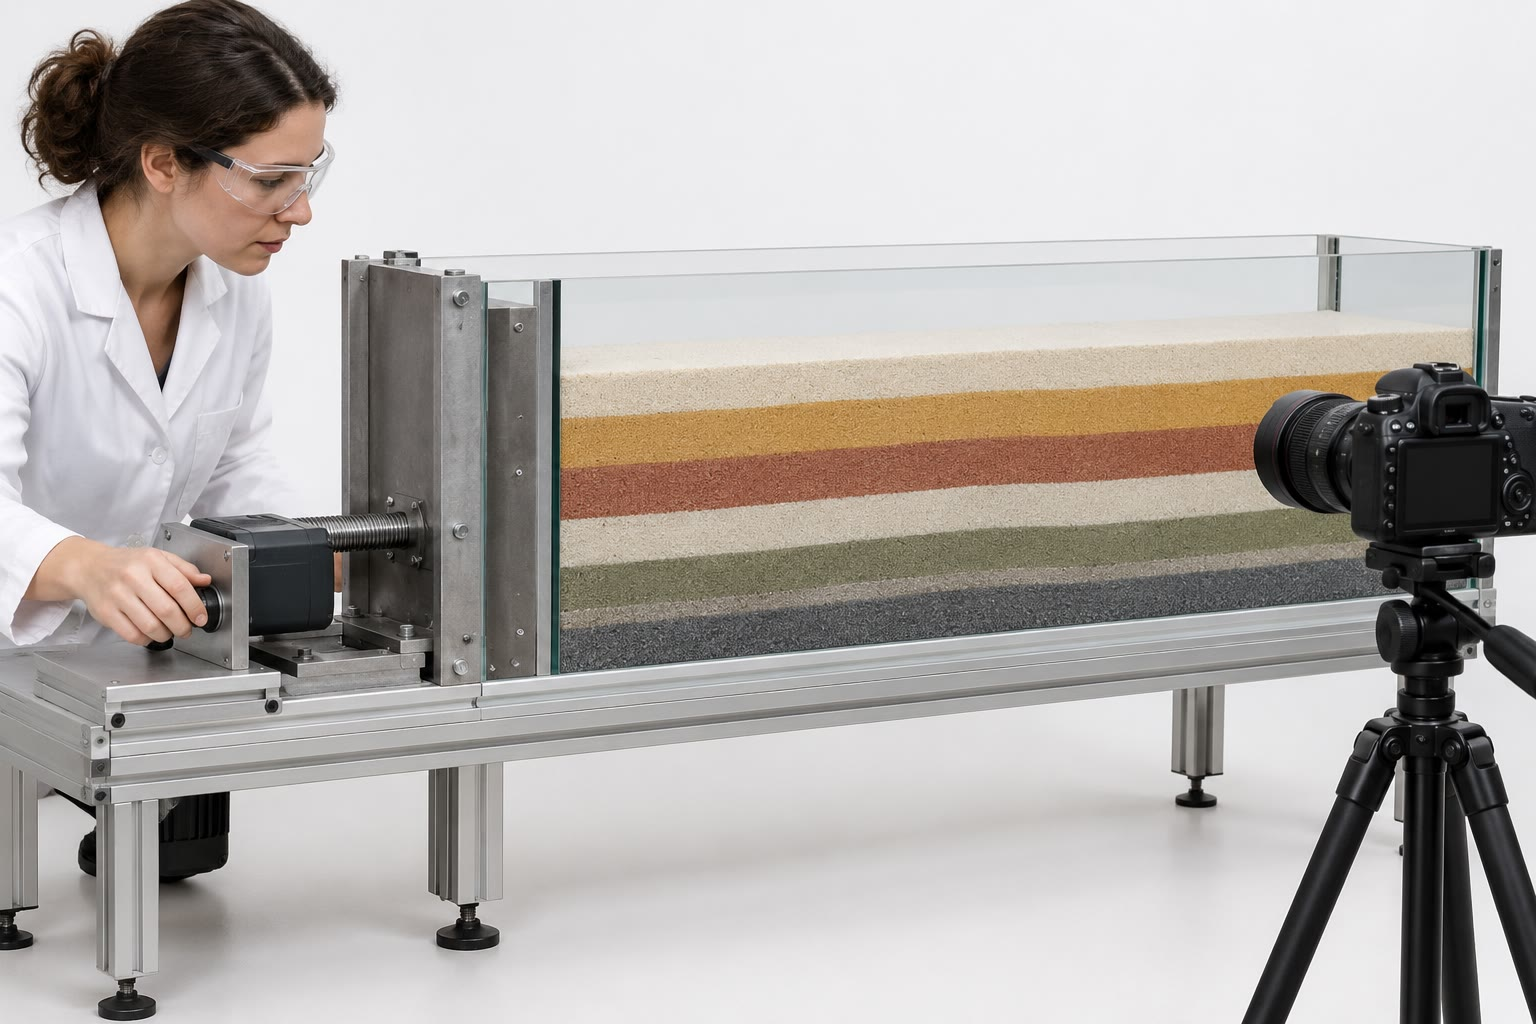
\includegraphics[width=\linewidth]{images/book5/ai/b3-sandbox-lab.jpg}

{\scriptsize نموذج صندوق رملي قبل التقصير: طبقات رملية ملوّنة في
صندوق ذي جوانب زجاجية، وجدارًا يحرّكه محرّك عند اليسار، وكاميرا على حامل ثلاثي
(رسم توضيحي مولَّد بالذكاء الاصطناعي).}
\end{minipage}
\end{inthelab}
% ledger: dsd83:taper

\section{الوشيعات الحقيقية}\label{sec:b3:orogenic-wedges:real}

في حزام الطيّات والصدوع الزاحفة النشط في غرب تايوان، ميلُ السطح،
وانحدار سطح الانفصال، والضغوط المسامية، كلّها معروفة من الطبوغرافيا،
والمقاطع الزلزالية والآبار. واستخدمها ديفيس وسوبي ودالن لحلّ
\omterm{thm:b3:orogenic-wedges:critical-taper}{معادلة الاستدقاق الحرج} لمقاومة الوشيعة، فوجدوا $\mu = 1.03$
داخل الكتلة و$\mu_b = 0.85$ عند القاعدة: احتكاك بايرلي عند القاعدة، ووشيعة أقوى من صدوعها،
لأنّ صدوعها ليست كلّها موجّهة للانزلاق
بسهولة. وبهذين المعاملين حوّلوا الاستدقاقات المرصودة لوشيعات نشطة أخرى، على اليابسة وتحت البحر،
إلى نسب للضغط المسامي، ووجدوها جميعًا فوق الضغط الهيدروستاتيكي،
بما يتّفق مع عمليات الحفر. ووجدوا أيضًا أين تتوقّف النظرية:
ينخفض الاستدقاق فجأةً حين تصبح الوشيعات أسمك من نحو
\qty{15}{km}، وهو العمق الذي تصبح عنده الصخور الغنية بالكوارتز لدنة
وفق المنحنيات الحرارية الشائعة، ولم تعد القاعدة تخضع لقانون احتكاكي.
% ledger: dsd83:taper

عند جبهة جبال الألب الغربية، تُعدّ الجورا وشيعةً زاحفة ذات زاوية ضيّقة
لا تتجاوز 3 إلى \ang{4}. ويقع سطح انفصالها في معظمه داخل طبقات حاوية للهاليت
من العصر الترياسي، والسوائل فيها ليست مفرطة الضغط: فضعف الملح وحده
يفسّر الاستدقاق الضيّق. وجنوب الجورا، حيث لا تحتوي الطبقات الترياسية على هاليت،
تبلغ الجبهة نفسها استدقاقًا من 12 إلى
\ang{13}، مع تراكمات من شرائح الصدوع الزاحفة، رغم أنّ ضغوط السوائل المقيسة
هناك مرتفعة. وفي جبال الألب الوسطى، يعطي تحليل \omterm{def:b3:orogenic-wedges:critical-taper}{الاستدقاق الحرج} لميل السطح
قيمةً للمقاومة القاعدية $\mu_b(1 - \lambda_b)$ (مع حدٍّ صغير للتماسك)
أدنى من 0.1، بل 0.05 في الصخور المتبخّرة والطَّفل قرب الجبهة،
وتزداد نحو الظهير الجبلي، مع نسب للضغط المسامي تفوق 0.54. تكون قاعدة الوشيعة غالبًا
أضعف بكثير مما يقتضيه قانون بايرلي، بحسب نوع صخرها
وبحسب سوائلها.
% ledger: deville21:jura, vonhagke14:alps

\section{الدفق عبر الوشيعة}\label{sec:b3:orogenic-wedges:flux}

تنمو الوشيعة عند استدقاقها الحرج بالتراكم، على شكل ثابت: يزداد طولها
وارتفاعها معًا. وتُزيل التعرية الصخر من سطحها. فحين
تتعادل العمليتان، تحافظ الوشيعة على حجمها، ويمرّ الصخر عبرها.

\begin{proposition}[توازن الدفق في الحالة المستقرّة]\label{prop:b3:orogenic-wedges:flux}
تستقبل وشيعة عرضها $W$ على امتداد اتجاه النقل، لكلّ وحدة طول
من الحزام، دفقَ التراكم $F_a = v h$، حيث $v$ هو معدّل التقارب
و$h$ سماكة الطبقة الواردة فوق سطح الانفصال. وتفقد
دفقَ التعرية $F_e = \bar e W$، حيث $\bar e$ هو متوسط معدّل التعرية
على سطحها. وتتغيّر مساحة مقطعها العرضي بمعدّل $F_a -
F_e$؛ وفي الحالة المستقرّة، $\bar e = vh/W$.
\end{proposition}

\begin{proof}
في وحدة الزمن، يعبر طولٌ $v$ من الطبقة الواردة، ذات السماكة $h$،
إلى داخل الوشيعة عبر طرفها، وتُزال السماكة $e(x)$ عند كلّ
نقطة من سطحها؛ والمساحة محفوظة، فتتغيّر مساحة المقطع
بمقدار $vh - \int_0^W e\,\mathrm dx = F_a - F_e$. وفي الحالة المستقرّة
يساوي التغيّر صفرًا.
\end{proof}

بأخذ $v = \qty{10}{mm/yr}$، و$h = \qty{4}{km}$، و$W = \qty{60}{km}$، فإنّ
معدّل التعرية اللازم للحالة المستقرّة هو $\qty{0.67}{mm/yr}$. والاستخراج
بالمعنى الوارد في مجلد السنة الثانية هو إزالة الصخر الذي يعلو صخرًا معيّنًا:
في الحالة المستقرّة، تبلغ الصخور السطح بالمعدّل الذي تُخفض به التعرية
سطحَه، وتُصعدها الوشيعة من أعماق كانت فيها ساخنة. ويتطلّب قياسُ
سرعةِ ذلك ساعةً تبدأ عند درجة حرارة معلومة.

\section{الكرونولوجيا الحرارية}\label{sec:b3:orogenic-wedges:thermochronology}

\begin{definition}[الكرونولوجيا الحرارية، الميقاتية الحرارية]\label{def:b3:orogenic-wedges:thermochronology}
\emph{الكرونولوجيا الحرارية}\index{الكرونولوجيا الحرارية} هي استخدام أعمار التبريد الإشعاعية
لتأريخ الزمن الذي مرّت فيه الصخرة بدرجة حرارة معيّنة،
ومن ثمّ إعادة بناء تاريخها الحراري. أمّا
\emph{الميقاتية الحرارية}\index{الميقاتية الحرارية} فهي زوج من معدن
وطريقة تأريخ مع درجة حرارة إغلاقها، مثلًا الأباتيت مع
طريقة \babelsublr{(U--Th)/He}، أو الزركون مع آثار الانشطار.
\end{definition}

يرتّب الجدول أدناه أهمّ الميقاتيات الحرارية بحسب درجة حرارة الإغلاق؛
تفترض الأعماق متوسّط درجة حرارة للسطح قدرها \qty{10}{\celsius}،
وتدرّجًا حراريًا منتظمًا قدره \qty{30}{\celsius/km}. والصخرة التي تبرد
أثناء استخراجها تمرّ بها تباعًا، وتتزايد أعمارها من الطرق منخفضة الحرارة
إلى الطرق مرتفعة الحرارة. أمّا الفيزياء الكامنة خلف آثار الانشطار وانتشار الهيليوم،
الذي يحدّد هذه الدرجات، فيرد في
\cref{ch:b3:advanced-geochronology}.
\begin{center}
\small
% ledger: sueoka19:closure
\begin{tabular}{lcc}
\hline
\omterm{def:b3:orogenic-wedges:thermochronology}{الميقاتية الحرارية} & درجة حرارة الإغلاق \babelsublr{(\unit{\celsius})} & العمق \babelsublr{(\unit{km})} \\
\hline
الأباتيت \babelsublr{(U--Th)/He} & \mbox{\textdir TLT 50--80} & \mbox{\textdir TLT 1.3--2.3} \\
آثار انشطار الأباتيت & \mbox{\textdir TLT 90--120} & \mbox{\textdir TLT 2.7--3.7} \\
الزركون \babelsublr{(U--Th)/He} & \mbox{\textdir TLT 160--200} & \mbox{\textdir TLT 5.0--6.3} \\
آثار انشطار الزركون & نحو 280 & 9 \\
\mbox{\textdir TLT \textsuperscript{40}Ar/\textsuperscript{39}Ar} على البيوتيت & \mbox{\textdir TLT 350--400} & \mbox{\textdir TLT 11--13} \\
\mbox{\textdir TLT \textsuperscript{40}Ar/\textsuperscript{39}Ar} على المسكوفيت & نحو 425 & 14 \\
U--Pb على الزركون & أعلى من 900 & --- \\
\hline
\end{tabular}
\end{center}

هذه الأعماق مجرّد تقدير أوّلي، لأنّ التعرية تغيّر المنحنى الحراري.

\begin{proposition}[المنحنى الحراري في الحالة المستقرّة مع التعرية]\label{prop:b3:orogenic-wedges:geotherm}
لترتفع صخرة بسرعة ثابتة $v$ عبر طبقة سمكها $L$، يُثبَّت سطحها ($z = 0$) عند $T_s$
وقاعدتها عند $T_L$، من دون أيّ إنتاج حراري.
وتكون درجة الحرارة المستقرّة:
\[
  T(z) = T_s + (T_L - T_s)\,\frac{1 - e^{-\mathrm{Pe}\,z/L}}{1 - e^{-\mathrm{Pe}}},
  \qquad \mathrm{Pe} = \frac{vL}{\kappa},
\]
ويساوي التدرّج عند السطح $\mathrm{Pe}/(1 - e^{-\mathrm{Pe}})$ مضروبًا في
التدرّج التوصيلي $(T_L - T_s)/L$.
\end{proposition}

\begin{proof}
تتحرّك جسيمة صخرية عند العمق $z$ نحو الأعلى، أي نحو قيم $z$ أصغر. فدرجة
الحرارة التي تحملها تتغيّر وفق $\partial T/\partial t - v\,\partial
T/\partial z$، وتصبح معادلة الانتشار $\partial T/\partial t - v
T' = \kappa T''$. في الحالة المستقرّة، $T'' = -(v/\kappa)T'$، إذن $T' = C
e^{-vz/\kappa}$، و$T = T_s + C(\kappa/v)(1 - e^{-vz/\kappa})$، وهذا يحقّق
$T(0) = T_s$. بوضع $T(L) = T_L$ يتحدّد $C$ فنحصل على الصيغة. عند $z =
0$، فإنّ $T' = (T_L - T_s)(\mathrm{Pe}/L)/(1 - e^{-\mathrm{Pe}})$.
\end{proof}

عندما $\mathrm{Pe} \ll 1$ يقترب المعامل من 1: يغلب التوصيل، ويبقى
المنحنى الحراري مستقيمًا. وعند $v = \qty{1}{mm/yr}$ عبر \qty{30}{km}، مع
$\kappa = \qty{e-6}{m^2/s}$، و$\mathrm{Pe} = 0.95$، ويرتفع التدرّج السطحي
من 30 إلى \qty{46}{\celsius/km}: تتزاحم خطوط التساوي الحراري نحو
السطح، وتُغلق كلّ ميقاتية حرارية عند عمق أقلّ.
% ledger: england:kelvin, earle:settings

\begin{definition}[علاقة العمر بالارتفاع]\label{def:b3:orogenic-wedges:age-elevation}
\emph{علاقة العمر بالارتفاع}\index{علاقة العمر بالارتفاع} لميقاتية حرارية هي
رسمُ أعمار التبريد لعيّنات جُمعت عبر مدًى من المناسيب،
عادةً على طول منحدر شديد أو مقطع رأسي،
بدلالة مناسيبها.
\end{definition}

\begin{proposition}[ميل علاقة العمر بالارتفاع]\label{prop:b3:orogenic-wedges:age-elevation}
لترتفع الصخور رأسيًا بسرعة ثابتة $v$ تحت طبوغرافيا مستقرّة،
ولنفترض أنّ خطّ تساوي درجة حرارة الإغلاق يقع عند المنسوب $e(x) = e_0 +
f\,h(x)$، حيث $h(x)$ منسوب السطح، و$0 \le f < 1$. عيّنةٌ
تُجمع عند السطح على المنسوب $h$ يكون عمرها $t = (h - e)/v$،
وتكون \omterm{def:b3:orogenic-wedges:age-elevation}{علاقة العمر بالارتفاع} خطًّا مستقيمًا ميله
\[
  \frac{\mathrm dh}{\mathrm dt} = \frac{v}{1 - f}.
\]
وعند خطّ تساوي حرارة مستوٍ، $f = 0$، ويكون الميل هو معدّل الاستخراج.
\end{proposition}

\begin{proof}
الصخرة التي تقع الآن على السطح عند $x$ عبرت خطّ تساوي درجة الإغلاق مباشرةً
الواقع أسفله، عند المنسوب $e(x)$، وقد ارتفعت منذ ذلك $h - e$ بالسرعة $v$:
$t = (h - e_0 - fh)/v = ((1 - f)h - e_0)/v$. ومنه $\mathrm dt/\mathrm dh =
(1 - f)/v$.
\end{proof}

\begin{omfigure}
\begin{tikzpicture}
\begin{groupplot}[group style={group size=2 by 1, horizontal sep=1.7cm},
  omrecord, width=0.47\linewidth, height=0.45\linewidth, title style={font=\small},
  legend style={font=\scriptsize, legend cell align=left}]
\nextgroupplot[title={(أ) علاقة العمر بالارتفاع}, xlabel={عمر الأباتيت \babelsublr{(U--Th)/He} \babelsublr{(\unit{Myr})}},
  ylabel={الارتفاع فوق المتوسط \babelsublr{(\unit{km})}}, xmode=log, xmin=0.1, xmax=10,
  log ticks with fixed point, xtick={0.1,0.2,0.5,1,2,5,10}, ymin=-1, ymax=1]
% computed in figdata/bachelor-3/age_elevation.py
\addplot[black, thick, densely dotted] table[x=a30, y=h] {figdata/out/bachelor-3-age_elevation-ages.dat};
\addplot[red!70!black, thick, densely dashed] table[x=a10, y=h] {figdata/out/bachelor-3-age_elevation-ages.dat};
\addplot[omDef, thick] table[x=a03, y=h] {figdata/out/bachelor-3-age_elevation-ages.dat};
\nextgroupplot[title={(ب) خطّ تساوي درجة الإغلاق}, xlabel={المسافة \babelsublr{(\unit{km})}},
  ylabel={الارتفاع فوق المتوسط \babelsublr{(\unit{km})}}, xmin=0, xmax=40, ymin=-3.3, ymax=1.2,
  legend style={at={(0.5,0.03)}, anchor=south, legend columns=2}]
\addplot[black!70, very thick] table[x=x, y=h] {figdata/out/bachelor-3-age_elevation-iso.dat};
\addlegendentry{السطح}
\addplot[black, thick, densely dotted] table[x=x, y=e30] {figdata/out/bachelor-3-age_elevation-iso.dat};
\addlegendentry{\qty{3}{mm/yr}}
\addplot[red!70!black, thick, densely dashed] table[x=x, y=e10] {figdata/out/bachelor-3-age_elevation-iso.dat};
\addlegendentry{\qty{1}{mm/yr}}
\addplot[omDef, thick] table[x=x, y=e03] {figdata/out/bachelor-3-age_elevation-iso.dat};
\addlegendentry{\qty{0.3}{mm/yr}}
\end{groupplot}
\end{tikzpicture}

\par\smallskip{\small استخراج مستقرّ تحت تضاريس جيبية
طول الموجة \qty{20}{km} وسعتها \qty{1}{km}، عند ثلاثة معدّلات،
أنماط الخطوط كما في مفتاح (ب) (نموذج من الرتبة الأولى؛ طبقة سماكتها \qty{30}{km}، والسطح عند \qty{10}{\celsius}،
\qty{30}{\celsius/km} دون تعرية، $\kappa = \qty{e-6}{m^2/s}$، معدّل
التناقص الحراري \qty{6.5}{\celsius/km}، ودرجة حرارة الإغلاق عند \qty{65}{\celsius}). (أ) العمر مقابل
الارتفاع: الميول هي 0.59، و2.5، و\qty{14}{mm/yr}، لا 0.3، و1، و3.
(ب) متساوي الحرارة \qty{65}{\celsius} يتبع التضاريس بدقّة أكبر كلّما
كان الاستخراج أسرع، إذ يرتفع أقرب إلى السطح.}\label{fig:b3:orogenic-wedges:age-elevation}
\end{omfigure}
% ledger: earle:settings, england:kelvin, ussa76:layers, sueoka19:closure

لا تكون متساويات الحرارة مستوية تحت التضاريس: فالسطح أبرد على القمم
منه في الوديان بمقدار معدّل التناقص الجوّي، لكنّ ذلك أقلّ بكثير مما
ستكون عليه الصخور عند الارتفاع نفسه تحت الأرض، أمّا متساويات الحرارة الضحلة
تتبع التضاريس بصورة مخفّفة. بالنسبة إلى طبوغرافيا جيبية بطول موجة
$\Lambda$ ومعدّل التناقص $\Gamma$، يعطي حلٌّ من الرتبة الأولى للمعادلة
المستقرّة ما يلي:
\[
  f = \frac{(G_0 - \Gamma)\,e^{-mz_c}}{G(z_c)},\qquad
  m = \frac{v}{2\kappa} + \sqrt{\Bigl(\frac{v}{2\kappa}\Bigr)^2 +
  \Bigl(\frac{2\pi}{\Lambda}\Bigr)^2},
\]
حيث $z_c$ هو عمق متساوي حرارة الإغلاق تحت متوسط السطح،
$G_0$ تدرّج السطح، و$G(z_c)$ التدرّج عند $z_c$ (مُسلَّم به؛
يختبره البرنامج الحاسوبي). يتلاشى الاضطراب مع العمق على
مسافة $1/m$، على الأكثر $\Lambda/2\pi$: الميقاتيات الحرارية منخفضة الحرارة،
التي تُغلق ضحلًا تتأثّر بالتضاريس أكثر من غيرها. يُظهر الشكل أعلاه التأثير
في الأباتيت \babelsublr{(U--Th)/He}.
% ledger: sueoka19:closure, ussa76:layers

لا يقيس مقطع العمر بالارتفاع معدّل الاستخراج إلا حيث تكون
متساوي حرارة الإغلاق مستويًا تحت التضاريس. وفي غير ذلك يبالغ في تقديره بعامل $1/(1 - f)$، وهو يبلغ
اثنين أو أكثر بالنسبة إلى الأباتيت \babelsublr{(U--Th)/He} ضمن تضاريس طول موجتها \qty{20}{km}.
تُصحِّح هذا الأثر الأعمارُ المأخوذة من عدّة ميقاتيات حرارية على العيّنات نفسها، والنماذج الحرارية
للتضاريس.

\section{التمارين}

\begin{exercise}[$\star$]\label{exo:b3:orogenic-wedges:1}
احسب $K$ ونسبة $\sigma'_1/\sigma'_3$ عند الانهيار لإسفين
له $\phi = \ang{30}$.
\end{exercise}

\begin{exercise}[$\star$]\label{exo:b3:orogenic-wedges:2}
إسفين من الرمل الجاف في صندوق رملي (حيث $\lambda = \lambda_b = 0$) له $\mu = 0.6$
داخله و$\mu_b = 0.3$ على قاعدته. احسب ميل السطح الحرج على قاعدة
أفقية، ثم على قاعدة منحدرة بمقدار \ang{3}.
\end{exercise}

\begin{exercise}[$\star$]\label{exo:b3:orogenic-wedges:3}
مع سطح عند \qty{10}{\celsius} وتدرّج قدره \qty{30}{\celsius/km}،
تحقّق من أعماق جدول درجات حرارة الإغلاق للأباتيت
\babelsublr{(U--Th)/He}، وأثر الانشطار للأباتيت، وأثر الانشطار للزركون. أيّ
ميقاتية حرارية تُستخدم لتأريخ الاستخراج من عمق \qty{5}{km}؟
\end{exercise}

\begin{exercise}[$\star$]\label{exo:b3:orogenic-wedges:4}
منحدر ارتفاعه \qty{2}{km} وينحدر بزاوية \ang{30}. احسب طوله الأفقي
وطوله على امتداد الانحدار. بكم يُرفع طبقةٌ من الجدار المعلّق بعد أن
عبرته كاملًا، وما الانزياح الذي ينقل حدّ القطع لأدنى
طبقة من قاعدة المنحدر إلى السطح المستوي العلوي؟
\end{exercise}

\begin{exercise}[$\star\star$]\label{exo:b3:orogenic-wedges:5}
باستخدام معاملات تايوان، احسب ميل السطح الحرج على قاعدة
منحدرة بمقدار \ang{6}، من أجل $\lambda = \lambda_b = 0.4$ و$0.9$. ماذا تُحدث
زيادةُ ضغط السائل في إسفين كان عند استدقاقه الحرج؟
\end{exercise}

\begin{exercise}[$\star\star$]\label{exo:b3:orogenic-wedges:6}
\omterm{def:b3:orogenic-wedges:thrust-folds}{طية انحناء الصدع} تقع فوق منحدر ارتفاعه \qty{1.5}{km}؛ وطبقةٌ فوق
السطح المستوي العلوي تُظهر مساحة زائدة قدرها \qty{6.0}{km^2}. احسب الانزياح. يقرأ زميل له
الطية نفسها بوصفها طية انفصال، والطبقة واقعة على بُعد \qty{3.0}{km} فوق
سطح الانفصال. ما التقصير الذي سيجده؟
\end{exercise}

\begin{exercise}[$\star\star$]\label{exo:b3:orogenic-wedges:7}
خذ $\mu = 0.6$ داخل كلٍّ من إسفين الجورا (الاستدقاق \ang{3.5}) والإسفين الواقع
جنوبه (الاستدقاق \ang{12.5})، و$\lambda = 0.4$ هيدروستاتيكي داخلهما،
وانحدارًا قاعديًا قدره \ang{2} لكليهما. احسب مقاومة القاعدة $\mu_b(1 -
\lambda_b)$ التي يتطلّبها كلّ استدقاق، وقارِنها ببيرلي $0.85$ عند الضغط
الهيدروستاتيكي. هل تتّسق النتيجة مع سطح الانفصال في
الهاليت أسفل الجورا؟
\end{exercise}

\begin{exercise}[$\star\star$]\label{exo:b3:orogenic-wedges:8}
تصعد الصخور بمعدّل \qty{1}{mm/yr} عبر طبقة سماكتها \qty{30}{km}، من
\qty{910}{\celsius} عند قاعدتها إلى \qty{10}{\celsius} عند السطح، مع
$\kappa = \qty{e-6}{m^2/s}$. احسب \omterm{def:b3:lithosphere-thermal-models:peclet}{عدد بيكليه الحراري}، والتدرّج السطحي،
وعمق متساوي الحرارة \qty{65}{\celsius}. قارِن بالعمق
دون تعرية.
\end{exercise}

\begin{exercise}[$\star\star$]\label{exo:b3:orogenic-wedges:9}
عيّنتان من المنحدر نفسه، عند 1200 و\qty{2000}{m}، لديهما أعمار الأباتيت
\babelsublr{(U--Th)/He} البالغة 3.4 و\qty{4.6}{Myr}. احسب معدّل الاستخراج الظاهري
يعطي نموذج حراري للتضاريس $f = 0.5$: فما المعدّل الحقيقي؟
\end{exercise}

\begin{exercise}[$\star\star\star$]\label{exo:b3:orogenic-wedges:10}
بيّن أنّه، من أجل $\lambda = \lambda_b$، ينعدم ميل السطح الحرج عند
انحدار قاعدي $\beta^* = \mu_b/K$ لا يعتمد على $\lambda$. احسب ذلك من أجل
تايوان. ماذا يحدث لإسفين تكون قاعدته أشدّ انحدارًا؟
\end{exercise}

\begin{exercise}[$\star\star\star$]\label{exo:b3:orogenic-wedges:11}
بيّن أنّه، من أجل طول موجة طويل جدًا واستخراج بطيء جدًا، تميل $f$ إلى
$1 - \Gamma/G$، حيث $G$ هو التدرّج المنتظم؛ قدّر ذلك من أجل $G =
\qty{30}{\celsius/km}$ و$\Gamma = \qty{6.5}{\celsius/km}$. ما هو عندئذ
ميل \omterm{def:b3:orogenic-wedges:age-elevation}{علاقة العمر بالارتفاع}؟ ومن أجل $v = \qty{1}{mm/yr}$ وقيم
التمرين~8 (حيث $z_c = \qty{1.21}{km}$، $G_0 = \qty{46.5}{\celsius/km}$،
$G(z_c) = \qty{44.7}{\celsius/km}$)، احسب $f$ من أجل أطوال موجة 5
و\qty{20}{km}.
\end{exercise}

\begin{exercise}[$\star\star\star$]\label{exo:b3:orogenic-wedges:12}
يتّسع إسفين عند استدقاقه الحرج $\alpha + \beta$ \omterm{def:b3:orogenic-wedges:accretion}{بالتراكم الأمامي} وحده، دون
تعرية، انطلاقًا من الدفق $F_a$. بيّن أنّ عرضه يتزايد وفق
$W = \sqrt{2F_at/\tan(\alpha + \beta)}$. مع $F_a = \qty{40}{km^2/Myr}$ واستدقاق \ang{6}،
ما عرض الإسفين بعد \qty{2}{Myr}، وكم يلزم من الزمن ليبلغ
\qty{60}{km}؟
\end{exercise}

\section{مسألة: جبهة إسفين كيسترل}

\begin{problem}[{مسألة نهاية الأسبوع --- التقصير والميكانيك والدفق
والاستخراج لإسفين الصدع الزاحف المختلق}]
\label{pb:b3:orogenic-wedges:1}
% values: calc/ch10.py; critical_taper.py; age_elevation.py; fault_bend.py
سلسلة كيسترل هي الجبهة المختلقة لحزام جبلي، وهو حزام طيّات وصدوع زاحفة
فوق اليابسة بعرض \qty{60}{km}، يُدفع بمعدّل \qty{10}{mm/yr} فوق مقدّمة
طبقتها الرسوبية سماكتها \qty{4.0}{km} فوق سطح انفصال في الطَّفل.
يتبع صدعه الزاحف الأمامي سطح الانفصال على بعد \qty{4.5}{km} تحت السطح، ثم يصعد
منحدرًا بانحدار \ang{25}، ويمتدّ على السطح المستوي العلوي
على عمق \qty{1.5}{km}. عند الجبهة يعلو السطح \qty{0.3}{km} فوق مستوى سطح البحر، وسطح الانفصال
\qty{4.0}{km} تحته؛ وعلى بعد \qty{60}{km} خلف الجبهة يبلغ السطح ارتفاع
\qty{2.4}{km}، ويقع سطح الانفصال
\qty{8.2}{km} تحت مستوى سطح البحر. خذ، كما في تايوان، $\mu = 1.03$ و$\mu_b =
0.85$، وكثافة الصخر \qty{2500}{kg/m^3}، وكثافة الماء \qty{1000}{kg/m^3}،
و$g = \qty{9.81}{m/s^2}$.

\medskip\noindent\textbf{الجزء الأول --- هندسة الصدع الزاحف.}
\begin{enumerate}
  \item احسب ارتفاع المنحدر، وطوله الأفقي، وطوله
        على طول الانحدار.
  \item بكم ارتفعت طبقة من الجدار المعلّق بعدما
        عبرت المنحدر بأكمله؟
  \item فوق المنحدر، تُظهر طبقة تقع فوق السطح المستوي العلوي مساحة فائضة
        قدرها \qty{16.5}{km^2} فوق مستواها الإقليمي. احسب الانزياح.
  \item ما المساحة الفائضة المتوقّعة لطبقة أكثر ضحالة؟ لو قُرئت الطيّة
        على أنّها طية انفصال فوق سطح الانفصال، والطبقة
        على ارتفاع \qty{4.0}{km} فوقه، فأيّ تقصير كان سيُعثر عليه؟
  \item خلف المنحدر، يُظهر مقطع زلزالي دوبلكسًا من أربعة أحصنة، طول كلّ
        منها الآن \qty{2.5}{km} على امتداد الصدع الزاحف القاعدي، مقطوعة من
        شرائح طولها \qty{6.0}{km}. احسب التقصير الذي تستوعبه الأحصنة، وقارنه
        بالانزياح على المنحدر الأمامي.
  \item تشكّلت الأحصنة بالتتابع. أيّها الأحدث، ولماذا
        يكون الصدع الزاحف السقفي مطويًّا؟
\end{enumerate}

\medskip\noindent\textbf{الجزء الثاني --- الاستدقاق.}
\begin{enumerate}[resume]
  \item احسب ميل السطح $\alpha$ وانحدار القاعدة $\beta$
        والاستدقاق.
  \item احسب سماكة الإسفين على بعد \qty{60}{km} خلف الجبهة. هل يمكن
        استعمال نظرية إسفين كولوم؟
  \item احسب $K$. ما ميل السطح الذي يملكه إسفين جاف على هذه القاعدة؟
  \item ما ميل السطح الذي سيكون له مع ضغط مائع هيدروستاتيكي في
        الإسفين وعلى قاعدته؟ هل الإسفين متّسق معه؟
  \item حُلّ \omterm{thm:b3:orogenic-wedges:critical-taper}{معادلة الاستدقاق الحرج} من أجل $\lambda = \lambda_b$.
  \item احسب الإجهاد الرأسي وضغط المائع والضغط
        الهيدروستاتيكي عند قاعدة الإسفين على بعد \qty{60}{km} خلف الجبهة.
  \item يخفض التصريف $\lambda$ إلى 0.7. احسب ميل السطح الحرج
        الجديد. كيف يستجيب الإسفين؟
\end{enumerate}

\medskip\noindent\textbf{الجزء الثالث --- الدفق.}
\begin{enumerate}[resume]
  \item احسب دفق التراكم لكلّ كيلومتر من الحزام.
  \item ما متوسط معدّل التعرية الذي يُبقي الإسفين في الحالة المستقرّة؟
  \item احسب حجم الصخر المتعرّى سنويًّا وكتلته
        على \qty{100}{km} من الحزام.
  \item إذا توقّفت التعرية، بأيّ سرعة سيتّسع الإسفين في البداية؟
  \item إذا جرى تصفيح نصف الطبقة الواردة تحت مؤخّرة
        الإسفين بدلًا من تراكمها عند جبهته، فهل سيتغيّر معدّل التعرية المتوسط
        في الحالة المستقرّة؟ أين ستتركّز التعرية؟
\end{enumerate}

\medskip\noindent\textbf{الجزء الرابع --- الساعة.}
خذ الطبقة سماكتها \qty{30}{km}، و\qty{10}{\celsius} عند متوسط السطح
(\qty{2.0}{km} فوق مستوى سطح البحر)، و\qty{910}{\celsius} عند قاعدتها، $\kappa
= \qty{e-6}{m^2/s}$، ودرجة حرارة الإغلاق \qty{65}{\celsius} للأباتيت
\babelsublr{(U--Th)/He}، ومعدّل تناقص الحرارة \qty{6.5}{\celsius/km}، وتضاريس
طول موجتها \qty{20}{km}. تعطي خمس عيّنات جُمعت على جانب واحد من وادٍ:
\begin{center}
\small
\begin{tabular}{lccccc}
\hline
الارتفاع \babelsublr{(\unit{km})} & 1.30 & 1.65 & 2.00 & 2.35 & 2.70 \\
عمر الأباتيت \babelsublr{(U--Th)/He} \babelsublr{(\unit{Myr})} & 1.60 & 1.83 & 2.07 & 2.30 & 2.54 \\
\hline
\end{tabular}
\end{center}
\begin{enumerate}[resume]
  \item باعتبار معدّل التعرية في السؤال 15 معدّلَ الاستخراج، احسب
        \omterm{def:b3:lithosphere-thermal-models:peclet}{عدد بيكليه الحراري} والتدرّج الحراري السطحي.
  \item احسب عمق متساوي حرارة الإغلاق تحت متوسط السطح،
        والتدرّج الحراري عنده.
  \item بافتراض متساوي حرارة إغلاق مستوٍ، ما العمر الذي تُعطيه عيّنة
        عند الارتفاع المتوسط؟ قارنه بالبيانات.
  \item احسب $m$ وعامل الانثناء $f$.
  \item أجرِ ملاءمةً بخطّ مستقيم على بيانات العمر بالارتفاع. ما
        معدّل الاستخراج الظاهري الذي يعطيه ميله؟
  \item صحّحه من أجل انثناء متساوي الحرارة.
  \item قارِن بالجزء الثالث، وأعطِ معدّل استخراج
        إسفين كيسترل.
\end{enumerate}
\end{problem}
